\chapter{Calculus Applications to Probability}

\section{Probability Density Functions}
Recall from the chapter \textit{Continuous Probability Distributions} that for 
a single variable, $X$, the likelihood that variable $X$ has a certain value, 
$x$, is given by the probability distribution function (PDF), $f(x)$. 
Additionally, the total area under a PDF is always 1. Mathematically, this is 
because the PDF is the derivative of the cumulative density function (CDF), 
which always starts at 0 and ends at 1. Logically, the area under the PDF from 
$x = a$ to $x = b$ represents the likelihood that $X$ will be between $a$ and 
$b$. 

\begin{mdframed}[style = important, frametitle = {Probability that $X$ lies 
between $a$ and $b$}]
For a single variable, $X$, with a continuous density function, $f(x)$, the 
probability that $X$ lies between $a$ and $b$ is given by:
$$P( a \leq X \leq b) = \int_a^b f(x)\,dx$$
\end{mdframed}

Suppose that we know the PDF for human body mass and we wanted to know the 
probability that a randomly-selected person has a body mass between 70 and 80 
kgs. That probability would be represented by the integral of the PDF from $x 
= 70$ to $x = 80$ (see figure \ref{fig:mass_PDF}). 

\begin{figure}[htbp]
    \centering
    \begin{tikzpicture}
        \begin{axis}[axis lines = center, xmin = 0, xmax = 120, ymin = 0, 
        xlabel = mass (kg), ylabel = probability, clip = false]
            \addplot[name path = A, blue, thick, domain = 70:80]{
            (1/(10*sqrt(2*3.14159)))*(2.718)^(-1*(x - 72)^2/(2*10)^2)};
            \addplot[name path = B, black, thin, domain = 70:80]{0};
            \addplot[blue, thick, domain = 1:120, samples = 100] {
            (1/(10*sqrt(2*3.14159)))*(2.718)^(-1*(x - 72)^2/(2*10)^2)};
            \addplot[blue!30, opacity = 0.4] fill between [of = A and B];
            \draw[black, thin, dashed] (70, 0) -- (70, 0.04);
            \draw[latex-] (70, 0.035) -- (65, 0.04) node[left] {70 kg};
            \draw[black, thin, dashed] (80, 0) -- (80, 0.035);
            \draw[latex-] (80, 0.03) -- (90, 0.04) node[right] {80 kg};
        \end{axis}
    \end{tikzpicture}
    \caption{The highlighted area is equal to the probability that a person 
    has a mass between 70 and 80 kgs}
    \label{fig:mass_PDF}
\end{figure}

If we expand that integral to include all possible masses, what would the 
integral evaluate to? Since that would represent the probability that a random 
person has mass (which all people do), the integral should be equal to 1. In 
fact, the integral of a PDF over all possible values of the variable must be 
equal to 1, since that represents the sum of all the probabilities that the 
variable will hold all possible values. 

\begin{mdframed}[style = important]
For any probability density function, $f(x)$, the integral over the domain of 
$x$ is always 1.
$$\int_{-\infty}^{\infty} f(x)\,dx = 1$$
\end{mdframed} 

\textbf{Example}: Let $f(x) = kx(10-x)$ for $0 \leq x \leq 10$ and $0$ for all 
other values of $x$. Find a value for $k$. Then find the probability that $x$ 
lies between 7 and 10. 

\textbf{Solution}: Since $f(x)$ is a PDF, we know that:
$$\int_{-\infty}^{\infty} f(x)\,dx = 1$$

Solving for $k$:
$$1 = \int_{0}^{10} kx(10-x)\,dx = k\int_0^{10} 10x - x^2\,dx$$
$$= k \left[5x^2 - \frac{1}{3}x^3 \right]_{x = 0}^{x = 10} = k\left[500 - 
\frac{1000}{3} \right] = k \left( \frac{500}{3} \right) = 1$$

Which implies that $k = \frac{3}{500} = 0.006$

Therefore, in order to be a PDF, $f(x) = 0.006x(10-x)$ and we can find the 
probability that $X$ lies between 7 and 10:
$$P(7 \leq X \leq 10) = \int_7^{10} 0.006x(10 - x)\,dx$$
$$= 0.006 \left[5x^2 - \frac{1}{3}x^3 \right]_{x = 7}^{x = 10} = 0.006 \left[ 
5 \left(100 - 49 \right) - \frac{1}{3} \left(1000 - 343 \right) \right]$$
$$= 0.006 \left[ 255 - \frac{657}{3} \right] = 0.006(36) = 0.216 = 21.6\%$$

Therefore, there is a 21.6\% chance that $X$ lies between 7 and 10. 

\begin{Exercise}[title = {Representing Probabilities as Integrals}, 
label = rep_int]
Let $f(t)$ be the probability density function for the time it takes you to 
complete your weekly chores at home. Express the following probabilities as 
integrals or state what the given integral represents in words. 
\begin{enumerate}
\item that you spend less that 15 minutes on your chores.
\item that you spend between half an hour and an hour on your chores.
\item that you spend more than 45 minutes on your chores. 
\item $\int_{20}^{\infty} f(t)\,dt$
\item $\int_{60}^{120} f(t)\,dt$
\end{enumerate}
\end{Exercise}

\begin{Answer}[ref = rep_int]
\begin{enumerate}
\item $\int_0^{15} f(t)\,dt$
\item $\int_{30}^{60} f(t)\,dt$
\item $\int_{45}^{\infty} f(t)\,dt$
\item the probability that you spend more than 20 minutes on your weekly 
chores.
\item the probability that you spend between 1 and 2 hours on your weekly 
chores.
\end{enumerate}
\end{Answer}

\begin{Exercise}[title = {Using PDFs to Find Probabilities}, label = int_pdf]
For each $f(x)$, find $k$ such that $f(x)$ is a PDF. Then, find the requested 
probability. 
\begin{enumerate}
\item $f(x) = 
\begin{cases}
\frac{ke^{2 - x}}{\left(1 + e^{2 - x} \right)^2},&-2 \leq x \leq 6\\
0,&\text{otherwise}
\end{cases}$, $P(X \geq 2)$
\item $f(x) = \frac{k}{2 + 4x^2}$, $P(1 \leq X \leq 4)$
\item $f(x) = k(6x - 3x^2)$ for $0 \leq x \leq 2$ and 0 otherwise, $P(X > 3/4)$
\vspace{95mm}
\end{enumerate}
\end{Exercise}

\begin{Answer}[ref = int_pdf]
\begin{enumerate}
    \item We know that
	$$1 = \int_{-\infty}^{\infty} f(x)\,dx = \int_{-2}^{6} \frac{ke^{2 - x}}{
	\left( 1 + e^{2 - x} \right)^2}\,dx$$

	Let $u = e^{2 - x}$, then $-du = e^{2 - x}dx$. Substituting:
	$$= \int_{x = -2}^{x = 6} \frac{-k}{\left(1 + u \right)^2}\,du = k \left[
	 \frac{1}{1 + u} \right]_{x = -2}^{x = 6} = k \left[ \frac{1}{1 + e^{2 - x}} 
	 \right]_{x = -2}^{x = 6}$$
	$$= k \left[ \frac{1}{1 + e^{-4}} - \frac{1}{1 + e^4} \right] = \frac{k \left(
	e^4 - 1 \right)}{1 + e^4} = 1$$

	Which implies that $k = \frac{1 + e^4}{e^4 - 1}$. Substituting for $k$, we 
	find the probability that $X \geq 2$ is:
	$$P(X \geq 2) = \frac{1 + e^4}{e^4 - 1} \int_2^6 \frac{e^{2 - x}}{\left( 1 + 
	e^{2 - x} \right)^2}\,dx = \frac{1 + e^4}{e^4 - 1} \left[ \frac{1}{1 + e^{2 - 
	x}} \right]_{x = 2}^{x = 6}$$
	$$= \frac{1 + e^4}{e^4 - 1} \left( \frac{1}{1 + e^{-4}} - \frac{1}{1 + 1} 
	\right) = \frac{1 + e^4}{e^4 - 1} \left(\frac{1}{1 + e^{-4}} - \frac{1}{2} 
	\right) \approx 0.5$$

	There is a 50\% chance the variable will be greater than 2. 

    \item We know that:
    $$1 = \int_{-\infty}^{\infty} \frac{k}{2 + 4x^2}\,dx = \frac{k}{2} \int_{-
    \infty}^{\infty} \frac{1}{1 + 2x^2}\,dx$$
    $$= \frac{k}{2} \left[ \frac{\arctan{(\sqrt{2}x)}}{\sqrt{2}} \right]_{x = -
    \infty}^{x = \infty} = \frac{k}{2} \left[ \frac{\arctan{(\infty)}}{
    \sqrt{2}} - \frac{\arctan{(-\infty)}}{\sqrt{2}} \right] $$
    $$= \frac{k}{2} \left( \frac{\pi}{2\sqrt{2}} - \frac{-\pi}{2\sqrt{2}} 
    \right) = \frac{k}{2} \left( \frac{\pi}{\sqrt{2}} \right) = \frac{\pi k}{2
    \sqrt{2}} = 1$$

    Which implies that $k = \frac{2\sqrt{2}}{\pi}$. Therefore $f(x) = \frac{
    \sqrt{2}}{\pi \left(1 + 2x^2 \right)}$. Additionally, 
    $$P(1 \leq X \leq 4) = \int_1^4 \frac{\sqrt{2}}{\pi \left(1 + 2x^2 \right)
    }\,dx = \frac{\sqrt{2}}{\pi} \int_1^4 \frac{1}{1 + 2x^2}\,dx$$
    $$= \frac{\sqrt{2}}{\pi} \left[ \frac{\arctan{(\sqrt{2}x)}}{\sqrt{2}} 
    \right]_{x = 1}^{x = 4} = \frac{1}{\pi} \left[ \arctan{(4\sqrt{2})} - 
    \arctan{(\sqrt{2})} \right] \approx \frac{0.441}{\pi} \approx 0.140 = 14\%$$

    \item We know that:
    $$1 = \int_{-\infty}^{\infty} k \left(6x - 3x^2 \right)\,dx = 3k \int_{0}^{
    2} 2x - x^2\,dx$$
    $$= 3k \left[x^2 - \frac{1}{3}x^3 \right]_{x = 0}^{x = 2} = 3k \left( 4 - 
    \frac{8}{3} \right) = 3k \left( \frac{4}{3} \right) = 4k = 1$$

    Which implies that $k = 1/4$. And therefore,
    $$P(X > \frac{3}{4} ) = \int_{3/4}^2 \frac{6x - 3x^2}{4}\,dx = \frac{3}{4} 
    \int_{3/4}^2 2x - x^2\,dx$$
    $$= \frac{3}{4} \left[ x^2 - \frac{1}{3}x^3 \right]_{x = 3/4}^{x = 2} = 
    \frac{3}{4} \left[ (2)^2 - \left( \frac{3}{4} \right)^2 - \frac{1}{3} 
    \left( 2^3 - \left( \frac{3}{4} \right)^3 \right) \right]$$
    $$= \frac{3}{4} \left( \frac{175}{192} \right) = \frac{175}{256} \approx 
    68.4\%$$
\end{enumerate}
\end{Answer}

\subsection{Exponential PDFs}
There are two common PDFs used to model real-world probability distributions: 
exponential and normal distributions. We address exponential PDFs in this 
section and will discuss normal PDFs in the next. 

The time it takes for a radioactive particle to decay, or a bank teller to 
serve a customer, or a piece of equipment to fail are all commonly modeled 
with exponentially decreasing PDFs. These take the form:
$$f(t) = 
\begin{cases}
0,&\text{if }t<0\\
ce^{-ct},&\text{if }t \geq 0
\end{cases}$$

\textbf{Example}: Carbon-14 has a half-life of 5700 years, and the probability 
that a single particle will undergo decay after a given amount of time, $t$, 
is given by:
$$f(t) = 
\begin{cases}
    0,\text{ if}t<0\\
    \frac{1}{5700}e^{-t/5700}&\text{if }t \geq 0
\end{cases}$$

Where $t$ is in years. Find the probability that a particle of carbon-14 
decays before 5700 years. 

\textbf{Solution}: 
$$P(T \leq 5700) = \int_0^{5700} \frac{1}{5700} e^{-t/5700}\,dt$$
$$= \frac{1}{5700} \left(-5700 \right) \left[e^{-t/5700} \right]_{t = 0}^{
t = 5700}$$
$$= -1 \left[ e^{-1} - e^{0} \right] = 1 - \frac{1}{e} \approx 63.5\%$$

\subsection{Normal Distributions}
Other natural phenomena, such as annual snowfall, height of individuals in a 
population, or birth weight are best modeled with a normal distribution. 
Professors often find that test scores are normally-distributed as well. 
Normal distributions have three key properties:
\begin{enumerate}
\item unimodal - there is one "peak" on a graph of a normal distribution
\item symmetric - there is an equal probability represented on either side of 
the "peak"
\item equal mean and median - the mean and median of a normal distribution are 
the same
\end{enumerate}

An example normal distribution is shown in figure \ref{fig:normal}. Notice 
that there is one peak and the graph is symmetric about that peak. 

\begin{figure}[htbp]
	\centering
	\begin{tikzpicture}
		\begin{axis}[xmin = -0.5, xmax = 20, ymin = 0, ymax = 0.2, 
		axis lines = center, xlabel = $x$, ylabel = $y$]
			\addplot[name path = A, blue, thick, fill = blue!30, opacity = 0.4, 
			domain = 0:20, samples = 300] 
			{1/(3*sqrt(2*3.14159))*e^(-(x - 10)^2/(2*3^2))};
            \draw[black, dashed] (10, 0) -- (10, 0.15) node[above] {mean = 10};
		\end{axis}
	\end{tikzpicture}
    \label{fig:normal}
    \caption{A normal distribution with a mean of 10 and a standard deviation 
    of 3}
\end{figure}

Normal PDFs take the form:
$$f(x) = \frac{1}{\sigma \sqrt{2\pi}} e^{-\left(x - \mu \right)/\left(2 
\sigma^2 \right)}$$

Where $\sigma$ is the \textit{standard deviation}\index{standard deviation} 
and $\mu$ is the \textit{mean}\index{mean}. Recall that for a normal 
distribution, the standard deviation is the distance you have to go from the 
mean to reach 68\% of the population. That is, if you look at the population 
within one standard deviation on either side of the mean, it represents 
approximately 68\% of the total population (see figure \ref{fig:stddev}). The 
lower $\sigma$ is, the narrower the distribution. The higher $\sigma$ is, the 
wider the distribution (see figure \ref{fig:stddevs}). 

\begin{figure}[htbp]
    \centering
    \begin{tikzpicture}
	\begin{axis}[xmin = -0.5, xmax = 20, ymin = 0, ymax = 0.2, axis lines = 
	center, xlabel = $x$, ylabel = $y$]
		\addplot[blue, thick, domain = 0:20, samples = 300] 
		{1/(3*sqrt(2*3.14159))*e^(-(x - 10)^2/(2*3^2))};
            \draw[red, dashed] (10, 0) -- (10, 0.15) node[above] {$\mu = 10$};
            \draw[black, dashed] (7, 0) -- (7, 0.11) node[above] {$\mu - 
            \sigma$};
            \draw[black, dashed] (13, 0) -- (13, 0.11) node[above] {$\mu + 
            \sigma$};
            \addplot[name path = A, blue, thick, domain = 7:13, samples = 200]
            {1/(3*sqrt(2*3.14159))*e^(-(x - 10)^2/(2*3^2))};
            \addplot[name path = B, domain = 7:13]{0};
            \addplot[fill = blue!30, opacity = 0.4] fill between [of = A and B];
		\end{axis}
	\end{tikzpicture}
    \label{fig:stddev}
    \caption{The shaded area represents approximately 68\% of the population}
\end{figure}

\begin{figure}[htbp]
    \centering
    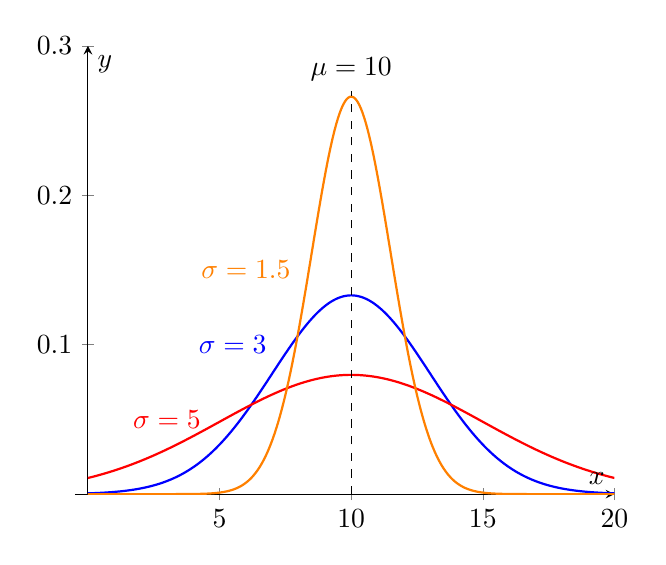
\begin{tikzpicture}
	\begin{axis}[xmin = -0.5, xmax = 20, ymin = 0, ymax = 0.3, axis lines = 
	center, xlabel = $x$, ylabel = $y$]
		\addplot[blue, thick, domain = 0:20, samples = 300] 
		{1/(3*sqrt(2*3.14159))*e^(-(x - 10)^2/(2*3^2))};
            \addplot[red, thick, domain = 0:20, samples = 300] 
            {1/(5*sqrt(2*3.14159))*e^(-(x - 10)^2/(2*5^2))};
            \addplot[orange, thick, domain = 0:20, samples = 300] 
            {1/(1.5*sqrt(2*3.14159))*e^(-(x - 10)^2/(2*1.5^2))};
            \node[orange] at (6, 0.15) {$\sigma = 1.5$};
            \node[blue] at (5.5, 0.1) {$\sigma = 3$};
            \node[red] at (3, 0.05) {$\sigma = 5$};
            \draw[black, dashed] (10, 0) -- (10, 0.27) node[above] {$\mu = 10$};
		\end{axis}
	\end{tikzpicture}
    \label{fig:stddevs}
    \caption{Changing $\sigma$ affects the width of the distribution, but not 
    its center}
\end{figure}

\textbf{Example}: Birth weights in the United States are normally distributed 
with a mean of 7 lbs 6 oz and a standard deviation 1 lb 2 oz. Write a PDF to 
represent this data. What percentage of US babies are born at less than 5 lbs? 
Over 9 lbs?

\textbf{Solution}: For simplicity, let's express everything in ounces. Recall 
that there are 16 oz in a pound. Therefore, 
$$\mu = 118\text{ oz}$$
$$\sigma = 18\text{ oz}$$

And we can write the PDF for US birth weight:
$$f(x) = \frac{1}{18\sqrt{2\pi}}e^{-\left(x - 118 \right)^2/\left(2 \left( 18 
\right)^2 \right)}$$

To find the percentage of babies with a birth weight below 5 lbs, we integrate 
from 0 (since a baby must have some weight) to 80 oz (the equivalent of 5 lbs):
$$P(X \leq 80) = \int_0^{80} \frac{1}{18\sqrt{2\pi}}e^{-\left(x - 118 \right)^2/
\left(2 \left( 18 \right)^2 \right)}\,dx$$

Unfortunately for us, there is no anti-derivative to $e^{-x^2}$, so we cannot 
evaluate the integral by hand. However, you can use a calculator or computer 
to find the approximate value of the integral. Inputting the integral into a 
calculator (such as a TI-89), we find that:
$$P(X \leq 80) \approx 0.0174$$

And therefore, approximately 1.74\% of US babies are born weighing less than 5 
lbs. 

To find the percentage of babies born weighing more than 9 lbs, we integrate 
from 144 oz to infinity (obviously, babies are not born with infinite weight, 
but this will do just fine for an approximation):
$$P(X \geq 144) = \int_{144}^{\infty} \frac{1}{18\sqrt{2\pi}}e^{-\left(x - 118 
\right)^2/\left(2 \left( 18 \right)^2 \right)}\,dx$$

Again, using a calculator or computer, we find that:
$$P(X \geq 144) \approx 0.0743$$

And therefore approximately 7.43\% of US babies are born weighing more than 9 
lbs. 

\section{Expected Value/Mean}
How can we find the average (mean) of a variable with a given probability 
distribution function? Consider the example of transaction processing times. 
If we knew the total time spent processing transactions and the total number 
of customers, then the mean processing time would be the total processing time 
divided by the total number of customers. 

Suppose we have a PDF that describes processing time for electronic 
transactions, $f(t)$, where $t$ is processing time and $f(t)$ is the 
probability that an individual transaction takes a particular amount of time, 
$t$. Electronic transactions are fast, and we can assume no transaction takes 
longer than 2 seconds, so we restrict the domain of $f(t)$ to $0 \leq t \leq 
2$. We can divide the PDF into intervals of width $\Delta t$ (see figure 
\ref{fig:mean}). 

\begin{figure}[htbp]
    \centering
    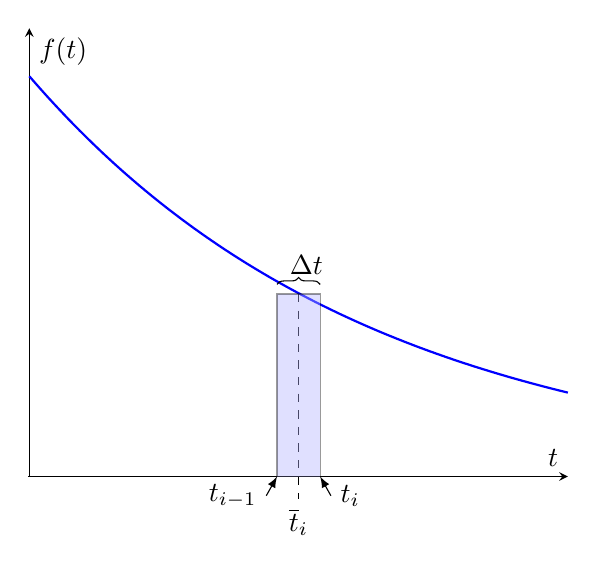
\begin{tikzpicture}
	\begin{axis}[xmin = -0.5, xmax = 250, ymin = 0, ymax = 0.007, axis lines = 
	center, xlabel = $t$, ylabel = $f(t)$, ticks = none, clip = false]
		\addplot[blue, thick, domain = 0:250, samples = 300] {(1/160)*e^(-1*x/160)};
        \draw[black, dashed] (125, 0.00285) -- (125, -0.00035) node[below] {
        $\overline{t}_i$};
        \draw[black, fill = blue!30, opacity = 0.4] (115, 0) rectangle 
        (135, 0.00285);
        \draw[latex-] (115, 0) -- (110, -0.0003) node[left] {$t_{i-1}$};
        \draw[latex-] (135, 0) -- (140, -0.0003) node[right] {$t_i$};
        \draw[decorate, decoration = brace] (115, 0.003) -- (135, 0.003) 
        node[above, xshift = -5] {$\Delta t$};
		\end{axis}
	\end{tikzpicture}
    \label{fig:mean}
    \caption{The probability that an individual transaction takes between 
    $t_{i-1}$ and $t_i$ seconds is approximated by the shaded area}
\end{figure}

If a total of $N$ transactions are processed, then the number of transactions 
that take between $t_{i-1}$ and $t_i$ is the probability of a transaction 
taking between $t_{i-1}$ and $t_i$ times $N$. That probability is approximately $f(\overline{t}_i) \Delta t$, and so the number of transactions taking between 
$t_{i-1}$ and $t_i$ is $Nf(\overline{t}_i) \Delta t$. Each of these 
transactions took approximately $\overline{t}_i$, and therefore the total 
processing time for these transactions is the number of transactions multiplied
by the processing time:
$$\overline{t}_i \left[ N f(\overline{t}_i) \Delta t \right]$$

To find the total processing time for all transactions, we would add up the 
total processing time for each interval:
$$\sum_{i = 1}^n N \overline{t}_i f(\overline{t}_i) \Delta t$$

And to find the average or mean processing time, we would divide this sum by 
the total number of customers, $N$:
$$\text{mean processing time} = \sum_{i = 1}^n \overline{t}_i f(\overline{
t}_i) \Delta t$$

Taking the limit as $n \to \infty$, the sum becomes an integral:
$$\text{mean processing time} = \int_0^2 t \cdot f(t)\,dt$$

Recall that we use $\mu$ to represent the mean. Therefore, for a general PDF, 
$f(x)$, the mean is given by:
$$\mu = \int_{-\infty}^{\infty} x \cdot f(x)\,dx$$

\textbf{Example}: Find the mean value of the general exponential PDF, 
$$f(x) = 
\begin{cases}
0,&\text{if }x < 0\\
ce^{-cx},&\text{if }x \geq 0
\end{cases}$$

\textbf{Solution}: Applying the definition of the mean:
$$\mu = \int_{-\infty}^{\infty} xf(x)\,dx = \int_0^{\infty} xce^{-cx}\,dx$$
$$= -xe^{-cx}|_{x = 0}^{x = \infty} - \int_0^{\infty} -e^{-cx}\,dx$$
$$= 0 + \left[-\frac{1}{c}e^{-cx} \right]_{x = 0}^{x = \infty} = \frac{1}{c}$$

And since $\mu = 1/c$, we can re-write the general exponential PDF in terms of 
the mean:
$$f(x) = 
\begin{cases}
0,&\text{if }x < 0\\
\mu^{-1}e^{-x/\mu},&\text{if }x \geq 0
\end{cases}$$

\begin{Exercise}[title = {Onset of Symptoms}, label = symptoms]
Researchers find that the time between infection by the COVID virus and the 
onset of symptoms can be described by the PDF:
$$f(t) = 
\begin{cases}
\frac{1}{595} te^{-0.04t},&\text{if }0 \leq t \leq 120\\
0,&\text{otherwise}
\end{cases}$$

What is the mean time between infection and the onset of symptoms?
\vspace{50mm}
\end{Exercise}

\begin{Answer}[ref = symptoms]
$$\mu = \int_{-\infty}^{\infty} tf(t)\,dt = \frac{1}{595} \int_{0}^{120} t^2 
e^{-0.04t}\,dt$$

Applying integration by parts, we set $f = t^2$ and $dg = e^{-0.04t}dt$, which 
means $df = 2t\text{ }dt$ and $g = -25e^{-0.04t}$. Substituting, 
$$\frac{1}{595} \int_{0}^{120} t^2 e^{-0.04t}\,dt = \left[ \frac{-25t^2 
e^{-0.04t}}{595} \right]_{t = 0}^{t = 120} - \int_{0}^{120} \frac{-50te^{-0.04t
}}{595}\,dt$$
$$= -\frac{72000 e^{-4.8}}{119} + \frac{10}{119} \int_0^{120} t e^{-0.04t}\,dt$$

We apply integration by parts again to evaluate the integral. Let $f = t$ and 
$dg = e^{-0.04t} dt$, which means $df = dt$ and $g = -25e^{-0.04t}$. 
Substituting:
$$\mu = -\frac{72000 e^{-4.8}}{119} + \left( \frac{10}{119} \right) \left[ 
\left( -25te^{-0.04t} \right)_{t = 0}^{t = 120} - \int_0^{120} -25e^{-0.04t}
\,dt \right]$$
$$= -\frac{72000e^{-4.8}}{119} + \left( \frac{10}{119} \right) \left[ -25(120)
e^{-4.8} + \int_0^{120} 25e^{-0.04t}\,dt \right]$$
$$= -\frac{72000e^{-4.8}}{119} - \frac{30000e^{-4.8}}{119} + \frac{250}{119} 
\int_0^{120} e^{-0.04t}\,dt$$
$$= -\frac{6000e^{-4.8}}{7} + \frac{250}{119} \left[ -25e^{-0.04t} \right]_{
t = 0}^{t = 120}$$
$$= -\frac{6000 e^{-4.8}}{119} - \frac{6250}{119} \left[e^{-0.04t} \right]_{
t = 0}^{t = 120} = -\frac{6000e^{-4.8}}{119} - \frac{6250}{119}e^{-4.8} + 
\frac{6250}{119}e^{-1} \approx 45.035$$

Therefore, the mean time until the onset of symptoms is approximately 45 hours. 
\end{Answer}

\section{Joint Density Functions}
Recall that you've learned about \textit{probability density functions} in a 
previous chapter. For some variable, $X$, with probability density function 
$f(x)$, the likelihood that $X$ lies between $a$ and $b$ is given by:
$$P(a \leq X \leq b) = \int_a^b f(x)\,dx$$

We can extend this to two random variables, $X$ and $Y$. A function that 
describes the distribution of both variables is called a \textit{joint 
density function}\index{joint density function}. In particular, the probability
that $X$ and $Y$ lie in a region $D$ is:
$$P((X, Y) \in D) = \iint_{\textit{D}} f(x,y)\,dA$$

Where $f(x, y)$ is the two-variable joint density function. Just like with one 
variable, all probabilities are positive and the sum of the probabilities of 
all possibilities must be 1. Mathematically, 
$$f(x, y) \geq 0$$
$$\iint_{\mathbb{R}} f(x, y)\,dA = \int_{-\infty}^{\infty} \int_{-\infty}^{
\infty} f(x, y)\,dx\,dy = 1$$

\textbf{Example}: Suppose the joint density function for $X$ and $Y$ is given 
by:
$$f(x, y) = 
\begin{cases}
C(3x + y),& \text{if }0 \leq x \leq 15\text{, }0 \leq y \leq 15\\
0,&\text{otherwise}
\end{cases}
$$

where $C$ is a constant. Find the value of $C$ and the likelihood that $X \geq 
Y$.

\textbf{Solution}: To find $C$, we take advantage of the fact that the sum of 
all probabilities is 1. Therefore,
$$1 = \int_0^{15} \int_0^{15} C(3x + y)\,dx\,dy = \int_0^{15} C \left[ \frac{3
}{2}x^2 + xy \right]_{x = 0}^{x = 15}\,dy$$
$$= \int_0^{15} C \left[ \frac{675}{2} + 15y \right]\,dy = C \left[ \frac{675}{
2}y + \frac{15}{2}y^2 \right]_{y = 0}^{y = 15}$$
$$= C \left[ \frac{10125}{2} + \frac{3375}{2} \right] = 6750C = 1$$

Which implies that $C = \frac{1}{6750}$.

To find the probability that $X \geq Y$, we note that this is represented by 
the region $R = \{(x, y)\text{ }|\text{ }0 \leq x \leq 15, 0 \leq y \leq x$. 
Then the likelihood that $X \geq Y$ is given by:
$$\frac{1}{6750} \int_0^{15} \int_0^x \left( 3x + y \right) \,dy\,dx = \frac{
1}{6750} \int_0^{15} \left[ 3xy + \frac{1}{2}y^2 \right]_{y = 0}^{y = x}\,dx$$
$$= \frac{1}{6750} \int_0^{15} \left(3x^2 + \frac{1}{2}x^2 \right)\,dx = \frac{
1}{6750} \left( \frac{7}{2} \right) \int_0^{15} x^2\,dx$$
$$= \frac{7}{13500} \left( \frac{1}{3} \right) \left[x^3 \right]_{x = 0}^{x = 
15} = \frac{7}{13500} \left( \frac{1}{3} \right) 15^3 = \frac{7 \cdot 3375}{3 
\cdot 13500} = \frac{7}{12}$$

And this answer makes sense, as it is less than 1. 

\begin{Exercise}[title = {Joint Density Functions}, label = joint]
The joint density function for a pair of random variables, $X$ and $Y$ is
$$f(x, y) = 
\begin{cases}
	ky(1 + 2x),& \text{if } 0 \leq x \leq 1\text{, }0 \leq y \leq 2\\
	0,&\text{ otherwise}
\end{cases}$$
\begin{enumerate}
\item Find the value of the constant, k.
\item Find $P(X \leq \frac{1}{2}, Y \leq 1)$.
\item Find $P(X + Y \geq 1)$.
\end{enumerate}
\vspace{70mm}
\end{Exercise}

\begin{Answer}[ref = joint]
\begin{enumerate}
    \item $$1 = \int_0^1 \int_0^2 ky\left(1 + 2x \right)\,dy\,dx = k \left[ 
    \int_0^1 1 + 2x\,dx \right] \cdot \left[ \int_0^2 y \,dy \right]$$
    $$= k \left[ \left(x + x^2 \right)_{x = 0}^{x = 1} \right] \cdot \left[ 
    \frac{1}{2} \left( y^2 \right)_{y = 0}^{y = 2} \right] = k \left( 2 \right)
    \left( \frac{1}{2} \right) \left(4 \right) = 4k$$

    If $4k = 1$, then $k = 1/4$. 

    \item $$P(X \leq \frac{1}{2}, Y \leq 1) = \int_0^{1/2} \int_0^1 \frac{1}{4}
    y \left(1 + 2x \right)\,dy\,dx$$
    $$= \frac{1}{4} \left[ \int_0^{1/2} \left(1 + 2x \right)\,dx \right] \cdot 
    \left[ \int_0^1 y\,dy \right] = \frac{1}{4} \left[ \left(x + x^2 \right)_{
    x = 0}^{x = 1/2} \right] \cdot \left[ \frac{1}{2} \left(y^2 \right)_{y = 0}
    ^{y = 1} \right]$$
    $$= \frac{1}{4} \left( \frac{1}{2} + \frac{1}{4} \right) \left( \frac{1}{2}
    \right) \left( 1 \right) = \frac{3}{32}$$

    \item If $X + Y \geq 1$, then $1 - X \leq Y \leq 2$ and 
    $$P(X + Y \geq 1 ) = \int_0^1 \int_{1 - x}^2 \frac{1}{4} y \left(1 + 2x 
    \right)\,dy\,dx$$
    $$= \frac{1}{4} \int_0^1 \left(1 + 2x \right) \frac{1}{2} \left[y^2 \right]
    _{y = 1 - x}^{y = 2}\,dx = \frac{1}{8} \int_0^1 \left(1 + 2x \right) \left(
    2^2 - \left(1 - x \right)^2 \right)\,dx$$
    $$= \frac{1}{8} \int_0^1 \left(1 + 2x \right) \left(3 + 2x - x^2 \right)\,
    dx = \frac{1}{8} \int_0^1 3 + 8x + 3x^2 - 2x^3\,dx$$
    $$= \frac{1}{8} \left[ 3x + 4x^2 + x^3 - \frac{1}{2}x^4 \right]_{x = 0}^{x 
    = 1} = \frac{1}{8} \left[3 + 4 + 1 - \frac{1}{2} \right] = \frac{1}{8} 
    \cdot \frac{15}{2} = \frac{15}{16}$$
\end{enumerate}
\end{Answer}

Often, two variables are independent of each other. If both variables are 
random, the joint density function for the two variables is the product of the 
two individual probability distributions. For example, if the probability 
distribution of an individual's height, $H$, is given by $f_1(h)$ and the 
probability distribution of an individual's blood pressure, $B$, is given by 
$f_2(b)$, then the joint probability function for height and blood pressure is 
$$f(h, b) = f_1(h)f_2(b)$$

\textbf{Example}: Sally is spending the day at Six Flags Over Georgia and is 
looking forward to riding several roller coasters. The wait time for the Great 
American Scream machine, $X$, is modeled by density 
function
$$f_1(x) = 
\begin{cases}
0,&\text{ if } x < 0\\
\frac{1}{45}e^{-x/45},&\text{ if } x \geq 0
\end{cases}$$

And the wait time for the Georgia Scorcher, $Y$, is modeled by density function
$$f_2(y) = 
\begin{cases}
0,&\text{ if } y < 0\\
\frac{1}{30}e^{-y/30},&\text{ if } y \geq 0
\end{cases}$$

What is the probability that she spends less than 45 minutes total waiting for 
the two rides?

\textbf{Solution}: Since the variables are independent, the joint density 
function for both wait times is:
$$f(x, y) = f_1(x) f_2(y) = 
\begin{cases}
    \frac{1}{1350}e^{-x/45}e^{-y/30},& \text{ if } x \geq 0, y \geq 0\\
    0,&\text{ otherwise}
\end{cases}$$

We want to know the probability that $X + Y < 45$, which is represented by the 
region, $R$, shown below.

\begin{center}
   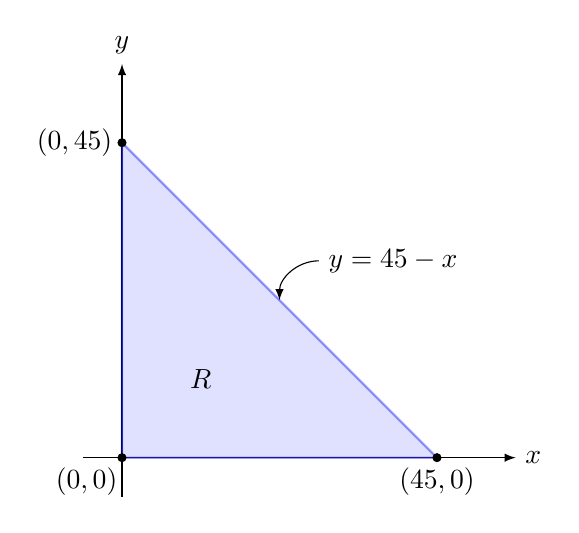
\begin{tikzpicture}
    \draw[-latex] (-0.5, 0) -- (5, 0) node[right] {$x$};
    \draw[-latex] (0, -0.5) -- (0, 5) node[above] {$y$};
    \draw[blue, thick, fill = blue!30, opacity = 0.4] (0,0) -- (0, 4) -- (4, 0)
     -- cycle;
    \draw[fill = black] (0,0) circle (0.05cm) node[below, xshift = -0.45cm] {
    $(0,0)$};
    \draw[fill = black] (4, 0) circle (0.05cm) node[below] {$(45, 0)$};
    \draw[fill = black] (0, 4) circle (0.05cm) node[left] {$(0, 45)$};
    \draw[latex-] (2, 2) arc [start angle = 180, end angle = 90, x radius = 
    0.5cm, y radius = 0.5cm] node[right] {$y = 45 - x$};
    \node[] at (1, 1) {$R$};
\end{tikzpicture}  
\end{center}

We can see that $R = \{(x, y)\text{ }|\text{ }0 \leq x \leq 45,\text{ }0 \leq 
y \leq 45 - x$. Therefore, the probability that Sally's total wait time is less
than 45 minutes is given by:
$$P(X + Y < 45) = \frac{1}{1350} \int_0^{45} \int_0^{45 - x} e^{-x/45} e^{-y/30
}\,dy\,dx$$
$$= \frac{-30}{1350} \int_0^{45} \left(e^{-x/45} \right) \left[e^{-y/30} 
\right]_{y = 0}^{y = 45 - x}\,dx$$
$$= -\frac{1}{45} \int_0^{45} \left( e^{-x/45} \right) \left[ e^{(x - 45)/30} 
- 1 \right]\,dx$$
$$= -\frac{1}{45} \int_0^{45} e^{(x - 135)/90} - e^{-x/45}\,dx$$
$$= -\frac{1}{45} \left[ 90e^{(x - 135)/90} + 45e^{-x/45} \right]_{x = 0}^{x = 
45}$$
$$= - \frac{1}{45} \left[ 90 \left( e^{(45 - 135)/90} - e^{(0 - 135)/90} 
\right) + 45 \left(e^{-45/45} - e^{-0/45} \right) \right]$$
$$= -\frac{1}{45} \left[90 \left( e^{-1} - e^{-3/2} \right) + 45 \left(e^{-1} 
- 1 \right) \right]$$
$$= -\frac{1}{45} \left[135e^{-1} - 90e^{-3/2} - 45 \right] = 1 + 2e^{-3/2} - 
3e^{-1} \approx 0.343$$

So, there is an approximately $34.3\%$ chance Sally will wait less than 45 
minutes to ride both roller coasters. 

\begin{Exercise}[title = {Snow Days}, label = snow]
In order for it to snow, two conditions must be met: the temperature must be 
low enough and the humidity must be high enough. The probability function for 
the temperature, $T$, in Celsius on a winter day is given by:
$$f_1(t) = 
\begin{cases}
    \frac{1}{80} \left[ \cos{\left( \frac{\pi t}{40} \right)} + 1 \right],& 
    -40 \leq t \leq 40\\
    0,&\text{otherwise}
\end{cases}
$$

And the probability function for the humidity, $H$, in percent on the same 
winter day is:
$$f_2(h) = 
\begin{cases}
    \frac{100h - h^2}{500,000},& 0 \leq h \leq 100\\
    0,&\text{otherwise}
\end{cases}
$$

If the temperature must be below freezing and the humidity above 75\% for snow 
to form, what is the probability it snows?
\end{Exercise}

\begin{Answer}[ref = snow]
The joint density function for temperature and humidity is:
$$f(t, h) = f_1(t)f_2(h) = \begin{cases}
    \frac{100h - h^2}{400,000,000}\left[ \cos{\left( \frac{\pi t}{40} \right)} 
    + 1 \right],& 0 \leq h \leq 100\text{, } -40 \leq t \leq 40\\
    0,&\text{otherwise}
\end{cases}$$

And the probability that snow forms is given by:
$$P(T \leq 0, 75 \leq H \leq 100) = \int_{-40}^{0} \int_{75}^{100} \frac{100h 
- h^2}{400,000,000}\left[ \cos{\left( \frac{\pi t}{40} \right)} + 1 \right]\,dh
\,dt$$
$$= \int_{-40}^0 \left(\frac{\cos{ \left( \frac{\pi t}{40} \right)} + 1}{
400,000,000} \right) \int_{75}^{100} \left(100h - h^2 \right)\,dh\,dt$$
$$= \int_{-40}^0 \left(\frac{\cos{ \left( \frac{\pi t}{40} \right)} + 1}{
400,000,000} \right) \left[ 50h^2 - \frac{h^3}{3} \right]_{h = 75}^{h = 100} 
\,dt= \int_{-40}^0 \left(\frac{\cos{ \left( \frac{\pi t}{40} \right)} + 1}{
400,000,000} \right) \left( \frac{78125}{3} \right)\,dt$$
$$= \frac{1}{15360} \int_{-40}^0 \left[ \cos{ \left( \frac{\pi t}{40} \right)} 
+ 1 \right]\,dt = \frac{1}{15360} \left[ \left( \frac{40}{\pi} \right) \sin{ 
\left( \frac{\pi t}{40} \right)} + t \right]_{t = -40}^{t = 0}$$
$$= \frac{1}{15360} (40) = \frac{1}{384} \approx 0.0026$$

So there is a 0.26\% chance it will snow. 
\end{Answer}

\section{Expected Values for Two Variables}
Recall that for one variable, $X$, the expected value of $X$ (its mean) is:
$$\mu = \int_{- \infty}^{\infty} xf(x)\,dx$$

Where $f(x)$ is the probability density function for $X$. Expanding this to two
independent random variables, $X$ and $Y$, we find the expected values for each
variable are:
$$\mu_x = \iint_{\mathbb{R}^2} xf(x, y)\,dA$$
$$\mu_y = \iint_{\mathbb{R}^2} yf(x, y)\,dA$$

\textbf{Example}: $X$ and $Y$ are random variables with joint density function:
$$f(x, y) = 
\begin{cases}
0.1e^{-(0.2x + 0.5y)},&\text{if } x \geq 0,\text{ }y \geq 0\\
0,&\text{otherwise}
\end{cases}$$

What are the expected values of $X$ and $Y$?

\textbf{Solution}: The expected value of $X$ is:
$$\mu_x = \int_0^{\infty} \int_0^{\infty} x(0.1)e^{-(0.2x + 0.5y)}\,dy\,dx$$
$$= \frac{1}{10} \int_0^{\infty} x \left(-2 \right) e^{-(0.2x + 0.5y)}|_{y = 0}
^{y = \infty}\,dx = -\frac{1}{5} \int_0^{\infty} (x)e^{-0.2x} \left[ e^{-0.5y} 
\right]_{y = 0}^{y = \infty}\,dx$$
$$= -\frac{1}{5} \int_0^{\infty} xe^{-0.2x} \left[ e^{-\infty} - e^0 \right]
\,dx = -\frac{1}{5} \int_0^{\infty} xe^{-0.2x} \left[0 - 1 \right]\,dx $$
$$= \frac{1}{5} \int_0^{\infty} xe^{-0.2x}\,dx$$

Applying integration by parts, 
$$\mu_x = \frac{1}{5} \left[ -5xe^{-0.2x}|_{x = 0}^{x = \infty} - \int_0^{
\infty} (-5)e^{-0.2x}\,dx \right]$$
$$= \left[-xe^{-0.2x} \right]_{x = 0}^{x = \infty} + \int_0^{\infty} e^{-0.2x}
\,dx  = -5e^{-0.2x}|_{x = 0}^{x = \infty}$$
$$= -5 \left(e^{-\infty} - e^0 \right) = -5 \left(0 - 1 \right) = 5$$

And the expected value of $Y$ is:
$$\mu_y = \int_0^{\infty} \int_0^{\infty} y(0.1)e^{-(0.2x + 0.5y)}\,dx\,dy$$
$$= \frac{1}{10} \int_0^{\infty} (y)e^{-0.5y} \int_0^{\infty} \left(e^{-0.2x} 
\right)\,dx\,dy = \frac{1}{10} \int_0^{\infty} (y)e^{-0.5y} \left[ -5e^{-0.2x} 
\right]_{x = 0}^{x = \infty}\,dy$$
$$= \frac{1}{10} \int_0^{\infty} (y)e^{-0.5y} \left(0 + 5 \right)\,dy = \frac{
1}{2} \int_0^{\infty} ye^{-0.5y}\,dy$$

Applying integration by parts:
$$\mu_y = \frac{1}{2} \left[(-2)ye^{-0.5y}|_{y = 0}^{y = \infty} - \int_0^{
\infty} (-2)e^{-0.5y}\,dy \right]$$
$$= \left[-ye^{-0.5y} \right]_{y = 0}^{y = \infty} + (-2)e^{-0.5y}|_{y = 0}^{y 
= \infty} = (-2) \left( e^{-infty} - e^0 \right) = -2(0 - 1) = 2$$

Therefore, the expected value of $X$ is 5 and of $Y$ is 2. 

\begin{Exercise}[title = {Expected Values}, label = expect]
The joint density function for a pair of random variables, $X$ and $Y$ is
$$f(x, y) = 
\begin{cases}
	\frac{1}{4} y (1 + 2x),& \text{if } 0 \leq x \leq 1\text{, }0 \leq y \leq 2\\
	0,&\text{ otherwise}
\end{cases}$$
What are the expected values of $X$ and $Y$?
\vspace{75mm}
\end{Exercise}

\begin{Answer}[ref = expect]
Finding the expected value of $X$:
$$\mu_x = \int_0^1 \int_0^2 \frac{1}{4}xy \left(1 + 2x \right)\,dy\,dx = 
\frac{1}{4} \int_0^1 x \left( 1 + 2x \right) \int_0^2 y\,dy\,dx$$
$$= \frac{1}{4} \int_0^1 x \left( 1 + 2x \right) \left[ \frac{1}{2} y^2 \right]_
{y = 0}^{y = 2}\,dx = \frac{1}{4} \int_0^1 x \left(1 + 2x \right) (2)\,dx$$
$$= \frac{1}{2} \int_0^1 x + 2x^2\,dx = \frac{1}{2} \left[ \frac{1}{2}x^2 + 
\frac{2}{3}x^3 \right]_{x = 0}^{x = 1}$$
$$= \frac{1}{2} \left( \frac{1}{2} + \frac{2}{3} \right) = \frac{1}{2} \left( 
\frac{7}{6} \right) = \frac{7}{12}$$

And finding the expected value of $Y$:
$$\mu_y = \int_0^2 \int_0^1 \frac{1}{4}y^2 \left(1 + 2x \right)\,dx\,dy = 
\frac{1}{4} \int_0^2 y^2 \int_0^1 \left( 1 + 2x \right)\,dx\,dy$$
$$= \frac{1}{4} \int_0^2 y^2 \left[x + x^2 \right]_{x = 0}^{x = 1}\,dy = 
\frac{1}{4} \int_0^2 y^2 (2)\,dy$$
$$= \frac{1}{2} \int_0^2 y^2\,dy = \frac{1}{2} \left[ \frac{1}{3}y^3 \right]_{
y = 0}^{y = 2} = \frac{1}{2} \left( \frac{1}{3} \right) (8) = \frac{4}{3}$$
\end{Answer}